\documentclass[12pt]{report}
\usepackage[utf8]{inputenc}
\usepackage{amsmath}
\usepackage{amsfonts}
\usepackage{amssymb}
\author{Edward Seabrook} 
\title{Third Year Project Progress Report}

\usepackage{titlesec}
\titleformat{\chapter}% reformat chapter headings
    [hang]% like section, with number on same line
    {\Large\bfseries}% formatting applied to whole
    {\thechapter}% Chapter number
    {0.5em}% space between # and title
    {}% formatting applied just to title

		\titlespacing*{\chapter}{0pt}{0pt}{20pt}

 %Get rid of margins?
 \usepackage[top=2.4cm, bottom=2.4cm, left=3.5cm, right=2.4cm]{geometry} 

\usepackage{todonotes}
\setlength{\marginparwidth}{3cm}
\reversemarginpar

\usepackage{hyperref}
\usepackage{listings}
\usepackage{appendix}
\usepackage{pdflscape}


\usepackage{fancyhdr} 
\pagestyle{fancy} 
\renewcommand{\headrulewidth}{0pt} 
\lhead{}\chead{}\rhead{}
\lfoot{}\cfoot{\thepage}\rfoot{}

\setcounter{secnumdepth}{3}
\setcounter{tocdepth}{3}

\begin{document}


\begin{titlepage}

\begin{center}


% Upper part of the page
%\includegraphics[width=0.15\textwidth]{./logo}\\[1cm]    

\LARGE Electronics and Computer Science\\
Faculty of Physical and Applied Sciences\\
University of Southampton
\\[1.5cm]

\href{mailto:ejfs1g10@ecs.soton.ac.uk}{Edward JF Seabrook}\\[0.5cm]

\today \\[1cm]
{\bfseries A Tool to Simplify Network Administration in the Modern Home}\\[1.5cm]

\vfill

% Author and supervisor
\large
Project Supervisor: 
Dr.~T \textsc{Chown}\\

\large
Secondary Examiner:
Dr.~KP \textsc{Zauner} 

\vfill

A Project Progress Report Submitted for the Award of Computer Science

\end{center}

\end{titlepage}



\begin{abstract}
\em No more than 200 words. \em


\end{abstract}

\tableofcontents
\clearpage
\listoftodos

\chapter{Project Description}
I left my initial project definition very open ended as I was undecided between
two projects. I was unsure of both the scope of a third year project, and my
competence as a software engineer. The original project definition was to create
``a tool to simplify network administration in the home''. The first potential
project was a home gateway monitoring system, the second was the project that
I have chosen. 

A more descriptive title for my project now is ``Implementing Zero configuration
OSPFv3''. I shall be augmenting an existing implementation of the OSPF (Open
Shortest Path First) network routing protocol such that it doesn't require any
configuration to effectively route network traffic on a simple multiple subnet
home network. The augmented implementation will be tested to ensure that it
works correctly both with homogeneous instances and instances of alternative
preexisting implementations. 

\section{Background}
As computing becomes more and more ubiquitous, home networks will have more and
more devices attached. It is difficult for us to predict all the possible future
uses of network devices; some examples might include sensor networks to monitor
the home, network attached appliances such as ovens and dishwashers and home
surveillance systems (e.g. CCTV). The IETF (Internet Engineering Task Force)
Home Networking (homenet) working group is doing a lot of exciting work into the
evolution of networking in residential homes. 

With an increasing number of devices, the traffic on the network will quickly
become very large. This is a problem that could be easily reduced by splitting
the network into multiple subnets. For example one for sensors, one for PCs and
one for appliances. 

It would also be a convenient way of enabling public access to a home network. A
subnet could be created for guests to connect to, either over wireless or some
form of Ethernet access point. The guest network could be provided with some
subset of the services of the main home network. Internet access could be
provided but file sharing protocols such as SMB (Server Message Block) would
still be unaccessible.

Routing technology is common place in larger networks such as Universities or
Businesses, where full time network administrators can be employed to set up and
maintain the networks. Unfortunately, most home users don't have much technical
knowledge, instead they demand a solution that can simply be plugged in and left
alone. This is where my project comes in. 



\todo{Where should I stick in the IPv4 vs IPv6 Spiel?}
Another problem that this project takes into consideration is the gradual
transition from 32bit Internet Protocol Version 4 (IPv4) to 128bit IPv6. As we
run out of IPv4 addresses, ISPs will be forced to start issuing IPv6 addresses
as IPv6 has as much larger number of possible addresses.

\section{Goals}
There are a number of goals that the project aims to meet, for it to be deemed
a success.

\subsection{Project Goals }
The following goals are things that the project should do:

\begin{itemize}
	\item Allow multiple networks in the home. And allow hosts on either
	network to communicate freely. 
	\item Require no configuration: The user shouldn't need to enter any 
	settings, they should simply plug in the router, and it should  work.
	\item Produce something of value for the community. The code I produce  
	should adhere to style and quality guidelines to ensure it is useful.
	\item Help to verify past implementations of the drafts.
	\item Discover any ambiguities in the drafts.
\end{itemize}

\subsection{Personal Goals}
By the end of the project I would like to have:

\begin{itemize}
	\item A better understanding of the process of the creation of internet
	standards.
	\item The ability to implement network protocols. 
	\item Improved programming skills (Mainly C or C++).
	\item Learned about new tools and techniques.
\end{itemize}

\chapter{Background and Literature Research}
The reading that I have done for this project can be split into two categories:
Theoretical reading which covers the theory behind the protocols, and Practical 
reading that covers the actual implementations to be used during the project.

\section{Theoretical Reading}
The majority of the information for this project is contained within various
RFCs (Request For Comments) and drafts of a similar nature. RFCs are memos
published by the IETF that are submitted for peer review. RFCs form the
standards that are used across the Internet. Where a more recent RFC has
obsoleted an older RFC, in this document, I shall tend to avoid mentioning the
older document. 

\subsection{RFC 2328} 
This RFC defines the OSPFv2 protocol, the protocol is a current internet
standard. It gives a complete description of the data structures and algorithms
of OSPF for IPV4. The appendices of the document provides the reader with a
clear understanding of the packets that are used in OSPF for IPv4. The author of
this RFC, J. Moy, has also written two books that continues the description. 

\subsection{RFC 5340}
This RFC defines the OSPFv3 protocol (OSPF for IPV6), the protocol is only a
proposed standard, but is very widely accepted.  Since OSPFv3 in general is
fairly similar to OSPFv2, the RFC describes only the differences between the two
protocols. 

\subsection{draft-dimitri-zospf-00}
This draft was published in 2002, and expired in 2003 - it never passed version
00.  However, it lays out many of the main concepts for later drafts.  A method
was proposed for running a cut down version of OSPFv3 for routing both IPv4 and
IPv6 traffic without requiring any manual configuration. 

\subsection{draft-ietf-ospf-ospfv3-autoconfig-00} 
This draft defines OSPFv3 Auto-Configuration, it is the main draft that will be
used for this project, it provides a set of modifications that can be made to
the OSPFv3 protocol to run (in a slightly restricted manner e.g.  single area)
it in without needing any manual configuration.  The draft discusses
configurations that should be set in some default manner, methods of selecting
Router-IDs (RID) and ways of detecting duplicate RIDs. 

The draft references many RFCs, a good understanding of the concepts 
that they convey is required to implement the draft successfully:

\begin{itemize}
	\item RFC 5838 - OSPFv3-AF (Address Families)
	\item RFC 6506 - OSPFv3-AUTH-TRAILER
	\item RFC 3630 (4230 \& 5786) - Traffic Engineering Extensions 
	\item RFC 4862 - SLAAC (IPv6) 
\end{itemize}


\subsection{draft-arkko-homenet-prefix-assignment-03}
 		
This draft is written by the same author as the previous draft, it defines
Prefix Assignment in Home Networks. As a testament to how recent this work is, a
new version of this draft has been released since the beginning of this project. 

The memo describes a method for dividing an IPv6 prefix across the subnets of a
home network using Type Length Values (TLVs) in OSPF Link State Advertisements
(LSAs).

\subsection{Cisco's Guide to Configuring OSPFv3}

Although it is aimed at network administrators rather than protocol
implementors, this document provides a nice high level overview of the OSPFv3
Protocol. I found it useful to use this document to understand the high level
concepts without having to worry about the low level details.

\subsection{OSPF: Anatomy of an Internet Routing Protocol}
 This book was written by the creator of OSPF (J. Moy). It defines the design
 and structure of OSPF in a greater level of detail than the RFC.

\subsection{OSPF: Complete Implementation}
The companion of the first book, also written by creator of OSPF. Gives a
complete implementation and walks you through how it has been put together. This
book and it's companion were written before OSPFv3.

\subsection{OSPF and IS-IS}
Talks about choosing an IGP (Interior Gateway Protocol) for large networks.
Makes a feature by feature comparison of OSPF with IS-IS (A similar distance
vector routing protocol). This book is mostly about OSPFv2 but does touch on
OSPFv3 towards the end.

\section{Practical Reading}		
Much of the practical information for this project is from online tutorials and
documentation of software projects.  

\subsection{Alix 2d3 Installation Guide}
This guide offered a comprehensive list of steps that need to be taken
to install Ubuntu linux on an Alix 2d3 board.  The article is written in
German but using Google translate I was able to follow it since a
large amount of it is Unix Shell commands.  

The process begins with installing the Compact flash card as a device on an
existing Ubuntu desktop PC. Next the card is partitioned using \texttt{fdisk},
the card is then formatted as ext2 (a linux filesystem type) using
\texttt{mk2fs}. The card is then mounted in the filesystem, using \texttt{mount}
and a small installation of Linux is copied to the card using
\texttt{debootstrap} to provide a base system.  

Several settings and devices are linked to the flash cards mount point and
\texttt{chroot} is used to simulate booting into the new install.

The required configuration files are edited (e.g. network interface settings)
and essential software packages (such as \texttt{vim}, \texttt{ssh},
\texttt{sudo}, and \texttt{apt}) are installed. A boot-loader such as
\texttt{grub} is also installed and configured.  Finally the Alix board is
booted with the flash card inserted.  

Using a USB to Null Model cable connected to the Alix board's serial port, a
terminal connection can be established using {\bf cu}. I had a few problems
using this device (\texttt{ttyUSB0}) but I was able to fix this problem using
\texttt{chown}. This terminal connection can be used to aide the boot process and ensure that
there are no Magic ELF errors. Once the Alix boards are up and running it is possible to
disconnect the serial cable and access them over \texttt{ssh} alone. 

\subsection{OSPF Implementations}
There are many different implementations of the OSPF protocol, the three most popular open
source implementations are XORP, Quagga and BIRD. Each of the projects appear to 
be well documented, hey all use Git as version control software and they all 
have somewhat active mailing lists (both user and developer).

\subsubsection{XORP}
XORP is an implementation of various routing protocols, including
OSPFv3. It is Implemented in C++ following an Object Oriented style.
OSPFv2 and OSPFv3 share much of the same code with conditional code
separating the parts which are different.

XORP implements OSPFv2 to comply with RFC2328 and OSPFv3 to the specification
defined in draft-ietf-ospf-ospfv3-update-23 (A draft version of RFC 5340).

\subsubsection{Quagga}
Quagga is another implementation of various routing protocols.  It is a
fork of the now defunct GNU Zebra project.  Quagga also implements
OSPFv3, taking a modular approach, providing a
completely seperate implementation of OSPFv2. The protocols are
implemented in C using a mainly Struct based style.  Vyatta the open
source software based virtual router notably switched from XORP to
Quagga. 

Quagga supports OSPFv2 as RFC 2328 and OSPFv3 to RFC2740. There are a few
differences between RFC2740 and RFC5240, these differences are listed in the
latter.

\subsubsection{BIRD}
BIRD is a more lightweight implementation. It also makes use of C
structs. It has already been used to successfully implement zero config OSPF. 
BIRD complies to RFC2328 and RFC5240 in it's implementations of OSPF. 

\chapter{Design of System}
\todo{The justification of approach should be included in this section IMO.}
Much of the design of my project has been done by individuals and groups of
people who have far more knowledge and experience working with networks than I
do. 

\section{Chosen System}
The routing protocol suite that I have chosen to base my project on is Quagga. I
made this choice for many reasons. Firstly, having been subscribed to the
mailing lists for a few weeks now, I observed that Quagga seems to be the most
active project. Secondly, Quagga splits up OSPFv2 and OSPFv3 - they do not share
any of the same source code; since I am only concerned with OSPFv3 for my
project, this should reduce some of the complexity involved with the
implementation. Quagga is also used by the Vyatta project (switching from XORP)
which gives it a large amount of exposure. 

I also found it easiest to install set up and use Quagga. It has a precompiled
package in Ubuntu's \texttt{apt} (Advanced Packaging Tool) repositories. One of
the reasons that I decided against using BIRD is that an implementation for a
new platform is more helpful to the community. One potential downside to using
Quagga is that it uses plain struct based C, and I have more experience writing
object oriented code. 

\begin{figure}
\caption{Diagram of how Quagga is structured.}
\centering
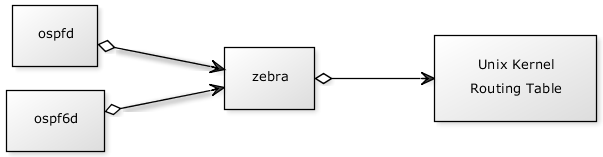
\includegraphics[width=\textwidth]{../Diagrams/UML/quaggaZebra.png}
\end{figure}


Quagga is split up into several daemons. A daemon is a a program that is run as
a background process rather than running interactively. Each of the daemons is
responsible for a single protocol. \texttt{ospfd} runs the OSPFv2 protocol, and
\texttt{ospf6d} runs the OSPFv3 protocol. Each of these daemons must go through 
\texttt{zebrad} to alter the systems routing table. 

As previously mentioned, Quagga is written in C and makes heavy use of
structs. The structs mimic object oriented programming, there is a struct for
each of the data structures defined in thd draft. 

\section{Test Networks}
To ensure that my changes work as expected, I will need to test instances of it
running on a few typical test networks. 

\missingfigure{Typical (future) home network topology(s)}

\chapter{Report on Technical Progress}
So far, I have made good progress on the project, and I am well on my way to
successfully completing the project by the final deadlines.


\section{Alix 2d3}
The Alix 2d3 boards have been set up to run Ubuntu Linux, a description of the
approach can be found above. In the future it may be necessary to create a more
customised build for these devices, if for example I find the performance to be
poor. So far they seem to have remained stable, both devices have an uptime of
over 28 days.

Quagga has been compiled and installed on one of the routers, and XORP on the
other. I installed BIRD to my desktop PC.  I found compilation of the projects on the machines themselves to be
very slow, so in the future I shall use a more powerful machine, for example a
desktop PC.

\section{Reading}
All of the material mentioned above has been read lightly. As many of the
documents reference the other documents, I found it difficult to fully
understand them, anything I am not confident about will be revisited once I have
a more solid foundation.

I have studied RFC 2328 (OSPFv2) and RFC 5340 (OSPFv3) in great depth making
detailed notes of their contents. I have also begun studying the appropriate
drafts.

As well as reading these documents, I have also looked at the source code of the
various implementation. After choosing to use Quagga, I began studying it's
source code in more depth to get an understanding of what changes need to be
made. 

\section{Network Topologies}
I have also begun to think about some network topologies that could be
used as test environments. These topologies need to test both typical home
networks, and stranger configurations that could result from inexperienced
people setting up the networks. 
 
As well as this I have begun attempting to assemble the networks that I have
suggested as test environments to ensure that I have sufficient hardware. 

\section{Progress Report}
Finally, I have written this document which has helped me formalise how my
project is coming along. Tasks such as creating a Gantt chart have helped me to
understand what I need to do when to stay on track.

\chapter{Plan of Remaining Work}
My project will continue throughout the Christmas holidays although I have
decided to plan as though I shan't be working over Christmas (or easter) to
ensure that I do have enough time to complete my project. The following tasks
need to be completed before I finish my project.

\section{Study Quagga}
I will need to study in depth the source code of Quagga so that I have a
good idea of what needs altering to implement the required changes. I will
produce Class diagrams and other UML (Unified Modelling Language) diagrams to 
summarise the architecture of the software. The process of producing these
diagrams should help ensure that I understand the code. I plan to start with the
diagrams above, and augment these to reflect the specified changes. 

\section{Implementation}
Next will come the main work of the project. I will need to perform the required
changes to augment the Protocol to conform with the drafts. I believe that this
section will take a large proportion of the time of the project, so I aim to
start this as early as possible. I shall begin by implementing as little as
is required to make it work, and then extending this in several iterations until
I have a complete product.

\section{Testing}
All projects require testing to ensure that they work as expected.

\subsection{Homogeneous Testing}
To verify that I have produced something that works, I shall test my
implementation homogeneously. I shall test it on the test network with all of
the routers running my implementation of zOSPF. 

\subsection{Heterogeneous Testing}
Networking protocols should not be implementation specific. As such, it should
be possible for my implementation to work harmoniously with one of the other
existing implementations. If they do not work together, this would indicate that
there is a problem with my implementation, the old implementation or there is an
ambiguity in the specification.

\subsection{User Testing}
As my project is intended to be used by home users, it might be useful to also
test on some actual users. The target audience would be technically able people
who have no experience of configuring multi-subnet networks. 

This would of course require ethics approval, so may not be possible.
\todo{Decide if I will test on people}

\section{Extensions}

The project is open to extensions.  There are a huge number of possible
extensions if I do finish early.

\subsection{Multiple Hop Service Discovery}
As my project would create the possibility to have multiple subnet, a possible
extension is to investigate, and potentially implement, the feasibility of
multiple hop service discovery. Essentially service discovery packets could be
forwarded by the routers of passed around inside the LSAs to enable a device on
one subnet to see a service advertised on another.

\subsection{Source Based routing}
It would also be possible to investigate source based routing. In a typical home
there is only one connection to the internet (Usually DSL) however, in the
future it may become more common for users to require two separate connections.
This could cause problems with traffic that needs to respond being sent to the
wrong gateway. Source based routing is a way of preventing this by inspecting
the source of the packet as well as it's destination.

\chapter{Project Management}

\section{Tool and Techniques}
\todo{Are there really any Techniques in here?}

During the project I shall be making use of many different tools and techniques
to help me complete various tasks. One of my goals is to learn about new tools,
so I have tried to use tools that I only have a small amount of experience
working with. 

\subsection{Git}
I have chosen to use Git as my version control system. This choice was
partially influenced by the fact that Quagga uses Git, however there are many
other good reasons for using Git, or any other Distributed Version Control
System (DVCS). Firstly, version control is essential to a software project as
it enables you to keep track of changes over time and revert to old versions if
neccessary. Distributed version control is superior to traditional centralised 
version control system such as SVN as it allows work to be done without internet
connectivity and speeds up commit time (hopefully encouraging more frequent
commits). I shall be using bit bucket to back up my repository in the ``cloud''.

\subsection{Trello}
I shall be using trello as a task management platform. Trello is a web app based 
on the Kanban method of project manaement. It provides card than can be placed
into lists and moved around between lists. Lists can have titles such as
``Thinking'', ``Doing'', ``Done''. Trello will help me to keep track of what
needs doing during my project.

\subsection{JIRA}
JIRA is an issue tracking software. I shall use it to keep track of bugs and
features that I need to work on. 

\subsection{Jenkins}
Jenkins is a continuous integration server, it can be configured to pull your
code from a repository and build it to make sure it still works.  

\subsection{\LaTeX}
I have chosen to produce all of the documentation associated with this project
using \LaTeX. I chose \LaTeX because it is a powerful tool that allows me to
focus on writing my report rather than typesetting. It also tends to be more
robust for longer documents than traditional WYSIWYG editors such as Microsoft
Word.

\subsubsection{Todonotes Package}
I have been using the package todonotes to help me keep track of ideas and tasks 
that need to be done in my documents. This gives me a nice way of keeping my
ideas separate from my finished work.

\subsubsection{Texcount}
As word counts are quite important throughout the project, I shall make use of
the texcount script to count the words in my documents. Texcount actually parses
the \LaTeX document so that markup and headings are not counted in the word
counts that it generated. 


\section{Gantt Chart}
No project would be complete without a Gantt chart... I'll try and find the one
from Christmas dinner last year...

\missingfigure{Gantt Chart}

\section{Risk Analysis}

When using the power supplied, there is a risk that I could get an electric
shock. I took the power supplies to be PAT tested on Zepler level 2. As the
power supplied are double insulated (i.e. no single failure can result in a
shock), a quick visual inspection by a trained member of staff reassured me that
they would be safe to use. 

Network outage. On the 1st - 2nd December 2012 ECS had a fairly major network
outage due to a hardware failure. I was unable to do other coursework because I
needed to use the software within ECS. Making use of a Distributed Version
Control System (DCVS) should help prevent this from being an issue. Replicate
code and resources in ECS, at home and in the cloud. 

\todo{When was the fire?}
There is a very real possibility of fire or some other unforeseeable damage to my
data, in 2005 the old Mountbatten building burned to the ground and a lot of
people lost work. To ensure that, if something like this happens, I will not be
affected, I shall make frequent backups of my work, using the aforementioned
source code control system.

As my project involves using specialist hardware, there is a possibility that
the hardware could break. Fortunately the operating system (Ubuntu) that is running on
the Alix boards is completely compatible with any x86 based computer. By adding
a second Network Interface Card to my desktop PC, I would be able to run the
software on there. 

It could turn out that I misjudged the difficulty of the project and I am not
able to complete in in the period of time available for a third year project.
Because of this I have chosen to structure my project in a modular way, with
different stages that I can attempt if I have time. This approach works quite
well as my project is fairly research based. 


\pagebreak


\begin{thebibliography}{9}

\addcontentsline{toc}{chapter}{Bibliography}

\bibitem{heartImg}
	Flickr Image of Heart \\
	gustty,\\
	\url{http://www.flickr.com/photos/gustty/126606794/}


\end{thebibliography}

\begin{landscape}
\appendix 
%\appendixpage

\chapter{Typical Home Networks}
\section{Present}
\begin{center}
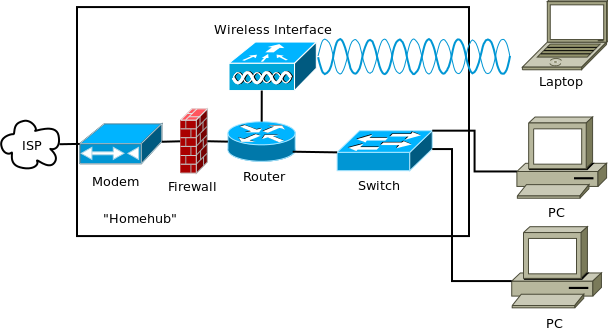
\includegraphics[width=0.75\linewidth]{../Diagrams/Network/TypicalHomenet.png}
\end{center}
This diagram shows a typical home network in the present day. The hardware
inside the box labeled ``Homehub'' is typically provided to the consumer in one
device which can simply be plugged in and should then just work. These devices
have many names, including ``Homehub'', ``Wirelessbox'', ``SuperHub'' and ``Home
gateway''. They are often also refered to as a router, although this is slightly
misleading as they perform many other tasks that routing. 

As can be seen from the diagram, the box provides the house with wireless and
wired connections to the LAN and the internet. The WLAN is typically bridged
with the LAN to give a single subnet to the user. 

\section{Future}
\begin{center}
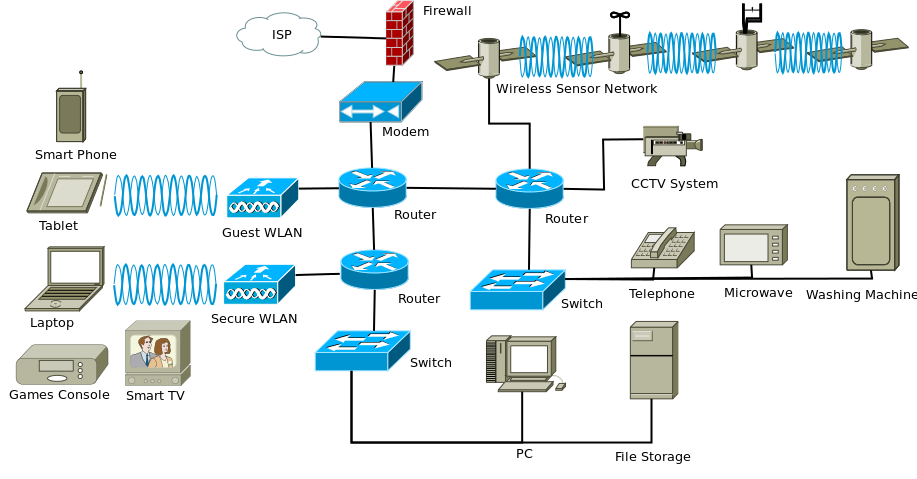
\includegraphics[width=0.9\linewidth]{../Diagrams/Network/FutureHomenet.png}
\end{center}
This diagram shows a hyperthetical future home network. The network includes a
guest wireless network, a secured wireless network, a wired network, a network
for applicances, a network for a home suveilence system and a wireless sensor
network. 


\end{landscape}
\end{document}

